\documentclass[a4paper,10pt]{article}

\usepackage{bm}
\usepackage{url}
\usepackage{bera}
\usepackage{epsfig}
\usepackage{comment} 
\usepackage{amsmath}
\usepackage{amssymb}
\usepackage{amsfonts}
\usepackage{hyperref}
\usepackage{listings}
\usepackage[T1]{fontenc}
\usepackage[margin=1.0in]{geometry}
\usepackage[square, comma, numbers, sort&compress]{natbib}

%opening
\title{Dynamical Many Body Freezing in the Kitaev Model}
\author{Analabha Roy}

\begin{document}

\maketitle
\section{\sc Introduction}
The Kitaev model, shown in fig~\ref{kitaev:lattice} has spin $1/2$'s on a honeycomb lattice, with highly anisotropic couplings between nearest neighbours. The dc Hamiltonian is
\begin{figure*}[hbt]
\ 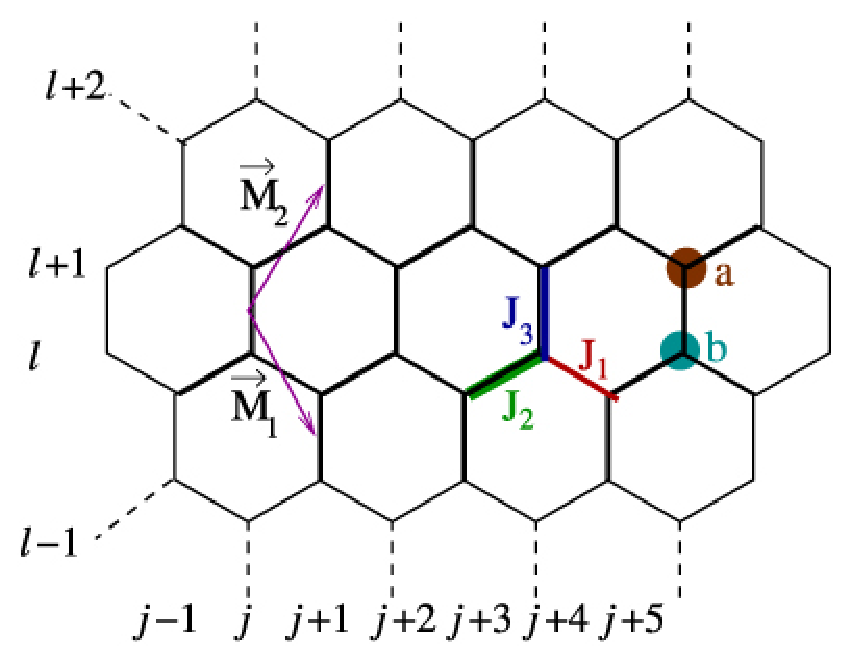
\epsfig{file=kitaev_model.eps,width=0.5\linewidth}
\caption{Kitaev model on a Honeycomb lattice}  
\label{kitaev:lattice}
\end{figure*}
\begin{equation}
\label{hamilt}
H = \sum_{j+l = {\rm even}} \left(J_1\; \sigma^x_{j,l}\sigma^x_{j+1,l}+J_2\;\sigma^y_{j-1,l}\sigma^y_{j,l}+J_3\; \sigma^z_{j,l}\sigma^z_{j,l+1}\right),
\end{equation}
where the couplings have nonnegative dc parts. This model can be solved exactly by mapping it to Majorana fermions by a Jordan-Wigner transformation. This allows for a block-diagonalization in momentun space to yield
\begin{eqnarray}
\label{hamilt:p}
H &=& \sum_{{\bf k}\in\mathcal{B}} 
\begin{pmatrix}
a^\dagger_{{\bf k}} & b^\dagger_{{\bf k}}
\end{pmatrix}
H_{{\bf k}}
\begin{pmatrix}
a^{\;}_{{\bf k}} \\
b^{\;}_{{\bf k}}
\end{pmatrix},\nonumber \\
H_{{\bf k}} &=& 2\left[J_3 + J_1 \cos{{\bf k}\cdot{\bf M}_1} + J_2 \cos{{\bf k}\cdot{\bf M}_2}\right]\sigma^z +\nonumber \\
	    & & 2\left[J_1 \sin{{\bf k}\cdot{\bf M}_1} - J_2 \sin{{\bf k}\cdot{\bf M}_2}\right]\sigma^x.
\end{eqnarray}
Here, $\mathcal{B}$ is the Brillouin zone indicated in fig~\ref{kitaev:fbz}, and $2\;{\bf M}_{1,2} = \sqrt{3} \hat{x}\pm 3\hat{y}$, shown in fig~\ref{kitaev:lattice}, and the operators $a_{\bf k}, b_{\bf k}$ are momentum representations of Majorana fermions that annihilate on the up-facing or down-facing 'y' sublattices respectively, as indicated in fig~\ref{kitaev:lattice}.
\section{\sc Driven Kitaev Model}
\begin{figure*}[hbt]
\ 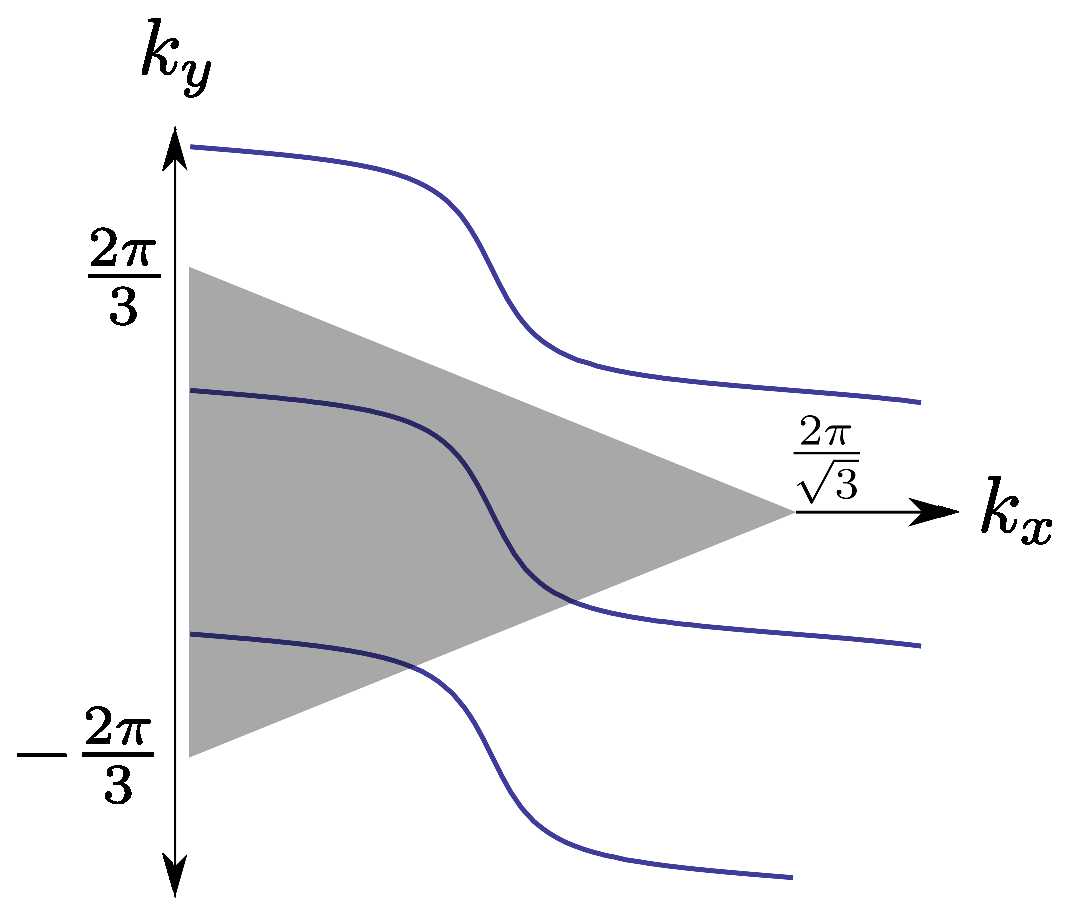
\epsfig{file=kitaev_fbz.eps,width=0.5\linewidth}
\caption{First Brillouin zone of Kitaev model indicated by gray triangle. The blue curves are loci of $\epsilon_{\bf k}=0$ for $J_1=0.6, J_2=0.4$.}  
\label{kitaev:fbz}
\end{figure*}
In this section, we introduce a periodic time dependence to the hopping $J_3 \rightarrow J_3 \sin{\omega t}$ with no dc part. The Schr\"odinger equation can be written as
\begin{eqnarray}
H_{\bf k}(t)|\psi_{\bf k}(t)\rangle &=& i \partial_t |\psi_{\bf k}(t)\rangle ,\nonumber \\
|\psi_{\bf k}(t)\rangle &=& \left[u_{\bf k}(t) + v_{\bf k}(t)a^\dagger_{\bf k}b^\dagger_{\bf k}\right]|0\rangle, \nonumber \\
H_{{\bf k}}(t) &=& 2\left(J_3 \cos{\omega t}+ J_1 \cos{{\bf k}\cdot{\bf M}_1} + J_2 \cos{{\bf k}\cdot{\bf M}_2}\right)\sigma^z +\nonumber \\
	       & & 2\left(J_1 \sin{{\bf k}\cdot{\bf M}_1} - J_2 \sin{{\bf k}\cdot{\bf M}_2}\right)\sigma^x,
\end{eqnarray}
and the full wavefunction $|\Psi(t)\rangle = \prod_{{\bf k}\in\mathcal{B}}|\psi_{\bf k}(t)\rangle$. This can be solved in the rotated basis using RWA to yield approximate solutions for large $\omega$. The Hamiltonian can be written as
$H_{\bf k}(t) = \left(\epsilon_{\bf k}+J_3\cos{\omega t}\right) \sigma^z + \Delta_{\bf k} \sigma^x$, with $\langle\psi_{\bf k}(t)|$ written in $SU(2)$ as $\left(u^\ast_{\bf k}(t), v^\ast_{\bf k}(t)\right)$, and $\epsilon_{\bf k}\equiv 2\left(J_1 \cos{{\bf k}\cdot{\bf M}_1} + J_2 \cos{{\bf k}\cdot{\bf M}_2}\right)$, $\Delta_{\bf k}\equiv2\left(J_1 \sin{{\bf k}\cdot{\bf M}_1} - J_2 \sin{{\bf k}\cdot{\bf M}_2}\right)$. We now transform to the rotated basis by the operator $U_{\bf k}(t)=e^{i\left(\epsilon_{\bf k}t+\frac{J_3}{\omega}\sin{\omega t}\right)\sigma^z}$, yielding the transformed Hamiltonian
\begin{eqnarray}
\label{rwa}
H'_{\bf k}(t) &=& U^{\;}_{\bf k}(t)H_{\bf k}(t)U^\dagger_{\bf k}(t)-i \bigg\{\partial_t U^{\;}_{\bf k}(t)\bigg\}U^{\dagger}_{\bf k}(t) ,\nonumber \\
	      &=& \Delta_{\bf k}\; U^{\;}_{\bf k}(t) \sigma^x U^{\dagger}_{\bf k}(t),\nonumber \\
	      &=& \Delta_{\bf k}\bigg\{e^{-2i\left(\epsilon_{\bf k}t+\frac{J_3}{\omega}\sin{\omega t}\right)}\sigma_+ + e^{2i\left(\epsilon_{\bf k}t+\frac{J_3}{\omega}\sin{\omega t}\right)}\sigma_-\bigg\},\nonumber \\
	      &\approx& \Delta_{\bf k} J_0(\eta) \bigg\{e^{-2i\epsilon_{\bf k}t}\sigma_+ + e^{2i\epsilon_{\bf k}t}\sigma_-\bigg\}.
\end{eqnarray}
In the last step above, we defined $\eta\equiv 2 J_3/\omega$, and expanded $e^{\mp i\eta\sin{\omega t}}=\sum_n J_n(\eta) e^{\mp i n \omega t}$, and took the rotating wave approximation, where we only considered the lowest-frequency contribution, as well as the resonance approximation, where the smallest mode is contributed by $n=0$ $\forall {\bf k}$ if $\omega\gg2\epsilon_{\bf k}$. The Schr\"odinger equation in the rotated wave basis (noting that $|\psi'_{\bf k}\rangle = U_{\bf k}(t)|\psi_{\bf k}(t)\rangle$) is
\begin{equation}
H'_{\bf k}(t)  |\psi'_{\bf k}\rangle = i\partial_t |\psi'_{\bf k}\rangle,
\end{equation}
and , with the approximations in eq~\ref{rwa}, can be solved exactly to yield
\begin{eqnarray}
u_{\bf k}(t) &=& e^{-i \epsilon_{\bf k}t } \bigg\{u_{\bf k}(0)\cos{\phi_{\bf k}t}+i\; \frac{\sin{\phi_{\bf k}t}}{\phi_{\bf k}} \left[u_{\bf k}(0) \epsilon_{\bf k} -\Delta_{\bf k}  J_0(\eta) v_{\bf k}(0)\right]\bigg\} , \nonumber \\
v_{\bf k}(t) &=& e^{i\epsilon_{\bf k}t } \bigg\{v_{\bf k}(0) \cos{\phi_{\bf k}t}-i\; \frac{\sin{\phi_{\bf k}t}}{\phi_{\bf k}} \left[\Delta_{\bf k}  J_0(\eta) u_{\bf k}(0)+v_{\bf k}(0) \epsilon_{\bf k} \right]\bigg\}, \nonumber \\
\end{eqnarray}
where $\phi_{\bf k}\equiv \sqrt{\epsilon^2_{\bf k}+J^2_0(\eta)\Delta^2_{\bf k}}$. A response like the expectation value of $\sigma_z$ is given by $m_{\bf k}(t)$, where
\begin{eqnarray}
 m_{\bf k}(t) &=& -1+ 2 |v_{\bf k}(t)|^2, \nonumber \\
              &=& 1- \frac{2J^2_0(\eta)\Delta^2_{\bf k}}{\epsilon^2_{\bf k}+J^2_0(\eta)\Delta^2_{\bf k}}\sin^2{\phi_{\bf k}t},
\end{eqnarray}
where we have started from all spins up at $t=0$ \textit{viz.} $u_{\bf k}(0)=0,v_{\bf k}(0)=1$. The time-momentum averaged response is thus
\begin{equation}
Q \equiv \lim_{n\rightarrow\infty}\frac{3\sqrt{3}\omega}{8\pi^3 n}\int^{2n\pi/\omega}_0 \mathrm{d} t \int_{{\bf k}\in\mathcal{B}}\mathrm{d}{\bf k}\; m_{\bf k}(t)\approx \frac{3\sqrt{3}}{4\pi^2}\int_{{\bf k}\in\mathcal{B}}\frac{\mathrm{d}{\bf k}\; \epsilon^2_{\bf k}}{\epsilon^2_{\bf k}+J^2_0(\eta)\Delta^2_{\bf k}},
\end{equation}
where we have approximately time-averaged $\sin^2{\phi_{\bf k}t}$ to $1/2$. The result above demonstrates that, provided $\epsilon_{\bf k}\neq0$, the magnetization freezes to unity when $J_0(\eta)=0$. However, the freezing is destroyed when $\epsilon_{\bf k}=0$. The locus of all such points in $\mathcal{B}$ is shown in fig~\ref{kitaev:fbz}. In the continuum limit, the measure contribution of the curve to the integral above is zero, and so the freezing is never destroyed. However, if $\epsilon_{\bf k}$ happens to be a constant, or weighed by a controllable parameter, then freezing is destroyed by the DC contribution whenever that parameter vanishes.


\end{document}
